\chapter{Конструкторская часть}

В данном разделе будут приведены схемы алгоритма обработки клиентских запросов.

\section{Сервер}

На рисунке \ref{fig:server} представлена схема алгоритма работы сервера, обслуживающего клиентские запросы с использованием сокетов.

В целях повышения масштабируемости приложения алгоритм работы сервера не зависит от подхода к параллельной обработке запросов. Добавить параллелизацию можно с использованием паттерна проектирования <<инъекция зависимостей>> (dependency injection).

\begin{figure}[H]
	\centering
	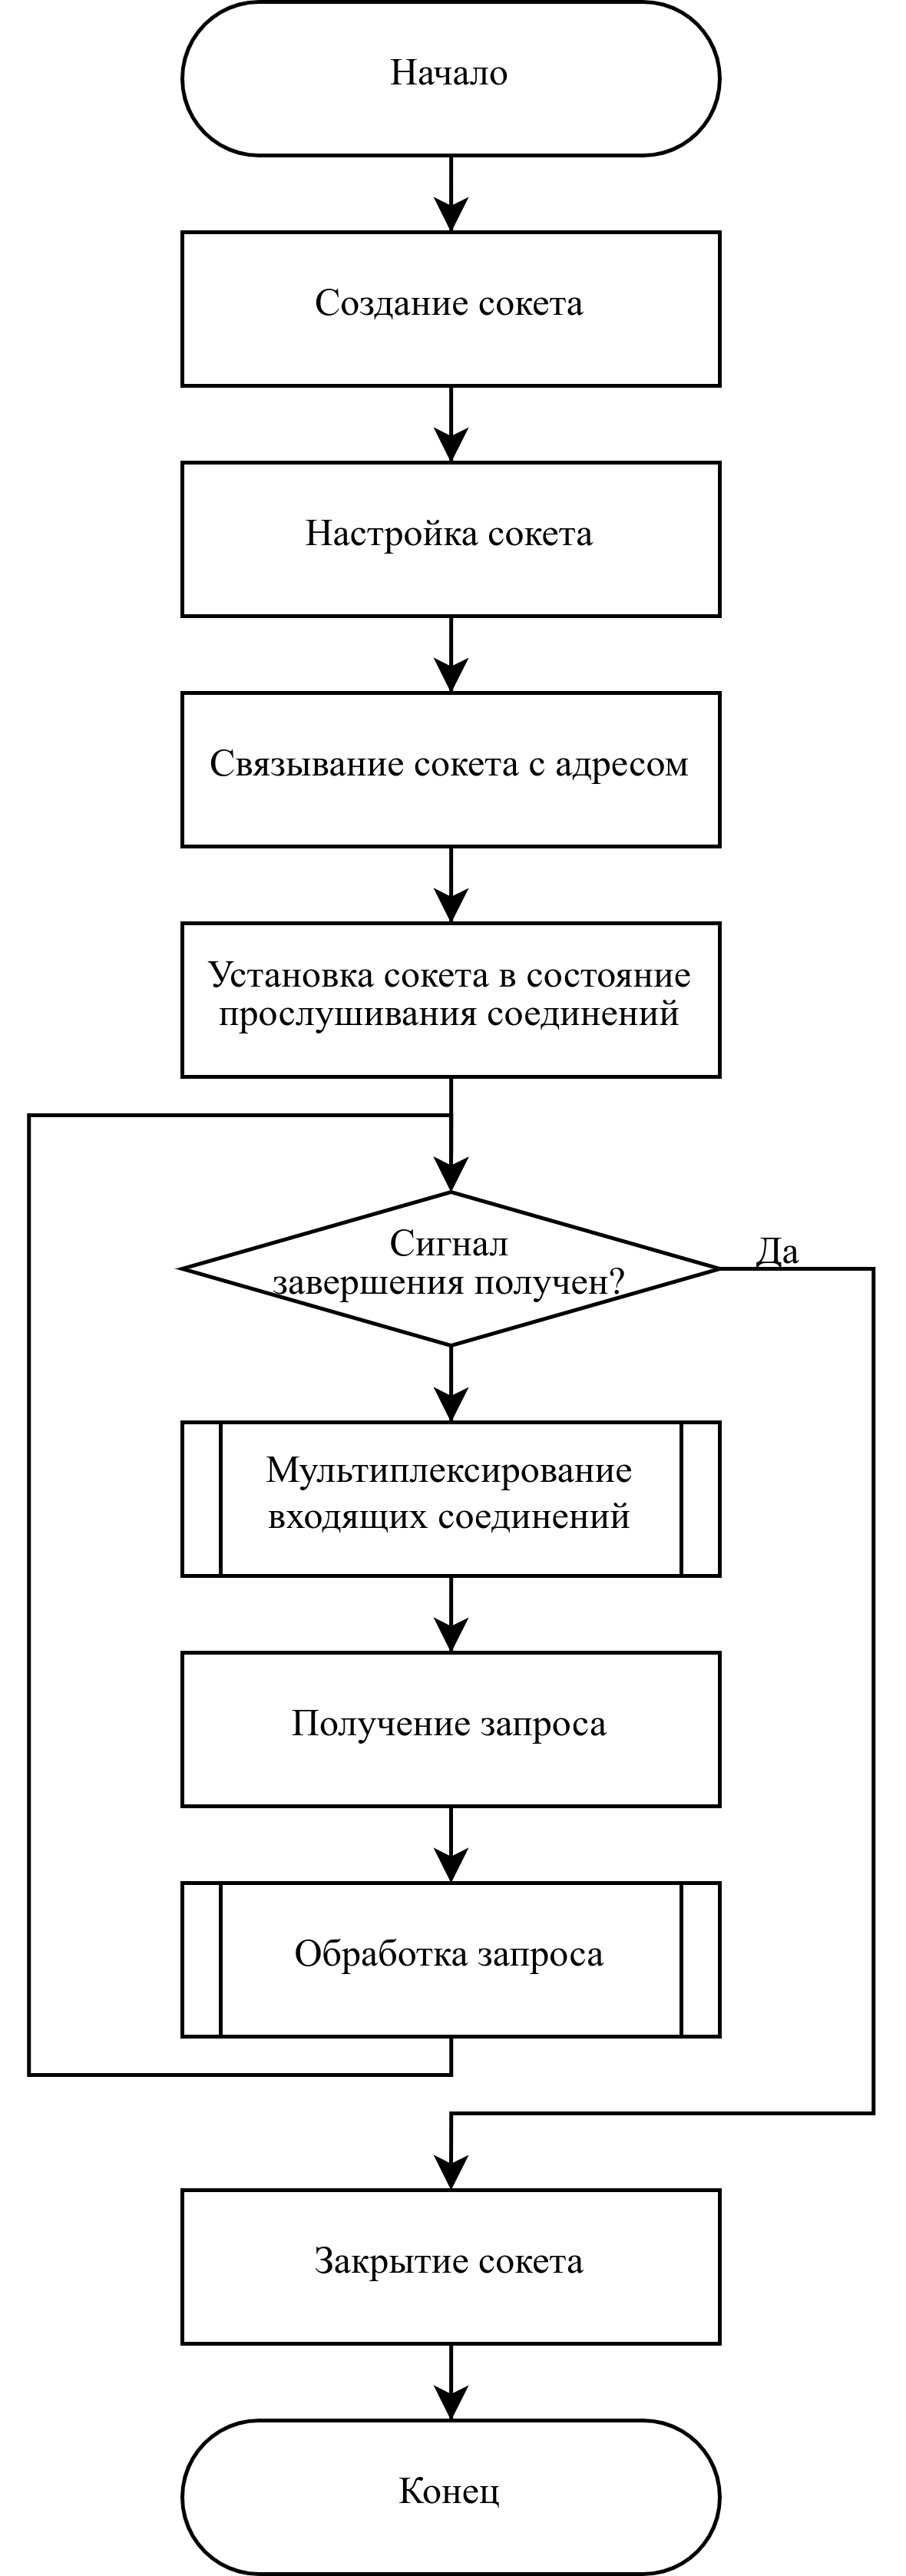
\includegraphics[scale=0.2]{assets/server.png}
	\caption{Алгоритм работы сервера}
	\label{fig:server}
\end{figure}



\section{Пул потоков}

На рисунке \ref{fig:pool} представлена схема алгоритма работы пула потоков.

\begin{figure}[H]
	\centering
	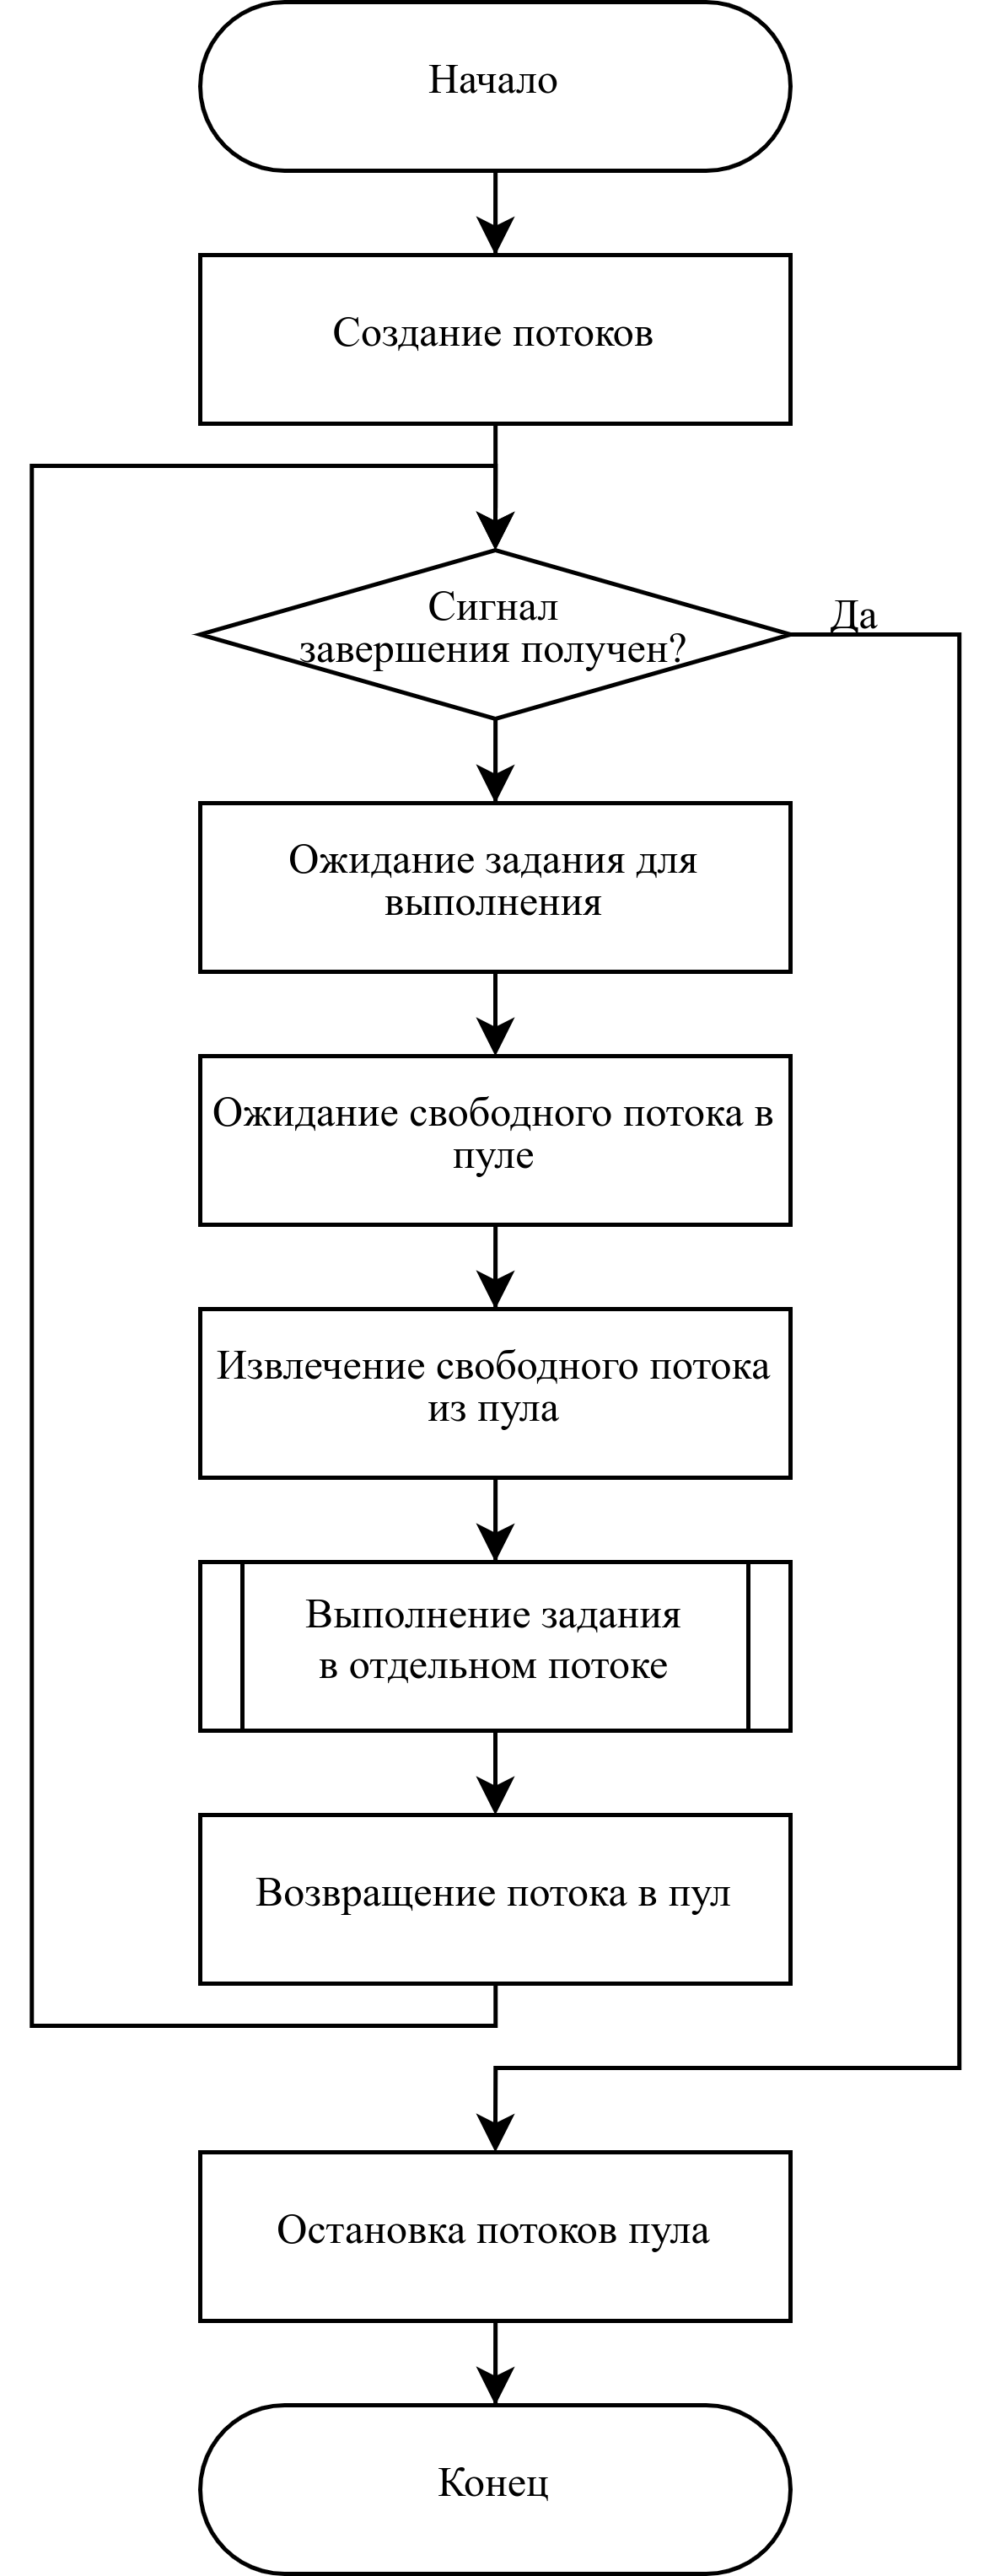
\includegraphics[scale=0.2]{assets/thread_pool.png}
	\caption{Алгоритм работы пула потоков}
	\label{fig:pool}
\end{figure}
